% ----------------------------------------------------------
% Teste test3_2_e25b32class2_20231211_231613
% ----------------------------------------------------------
\subsubsection{Teste test3_2_e25b32class2_20231211_231613 - AlexNet (Is That a Santa)}

Informações utilizadas para o treinamento.

\begin{table}[ht]
   \centering
   \caption{Treinamento}
   \label{tab:modelos}
   \begin{tabular}{| c | c | }
      \hline 
      \textbf{Informação} & \textbf{Descrição} \\
      \hline \hline 
      Rede & AlexNet \\
      \hline
      Número de épocas & 25\\
      \hline
      Tamanho do lote & 32\\
      \hline
      Taxa inicial & 0.012 \\
      \hline
      Taxa de decaimento & 0.0006 \\
      \hline
      Total de classes & 2\\
      \hline
      Dataset & CIFAR-10\\
      \hline
   \end{tabular} 
\end{table}

Resultados obtidos após treinamento.

\begin{tabular}{lrrrr}
\toprule
  Unnamed: 0 &  precision &   recall &  f1-score &    support \\
\midrule
       Santa &   0.913043 & 0.957655 &  0.934817 & 307.000000 \\
   Not Santa &   0.955479 & 0.908795 &  0.931553 & 307.000000 \\
    accuracy &   0.933225 & 0.933225 &  0.933225 &   0.933225 \\
   macro avg &   0.934261 & 0.933225 &  0.933185 & 614.000000 \\
weighted avg &   0.934261 & 0.933225 &  0.933185 & 614.000000 \\
\bottomrule
\end{tabular}


\begin{figure}[ht]
 \begin{center}
   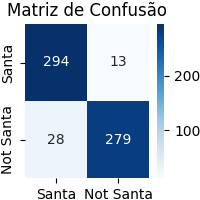
\includegraphics[scale=1]{tests/test3_2_e25b32class2_20231211_231613/confusion_matrix.png}
  \caption{Matriz de Confusão}
  \label{fig:fig03}
 \end{center}
\end{figure}

\begin{figure}[ht]
 \begin{center}
   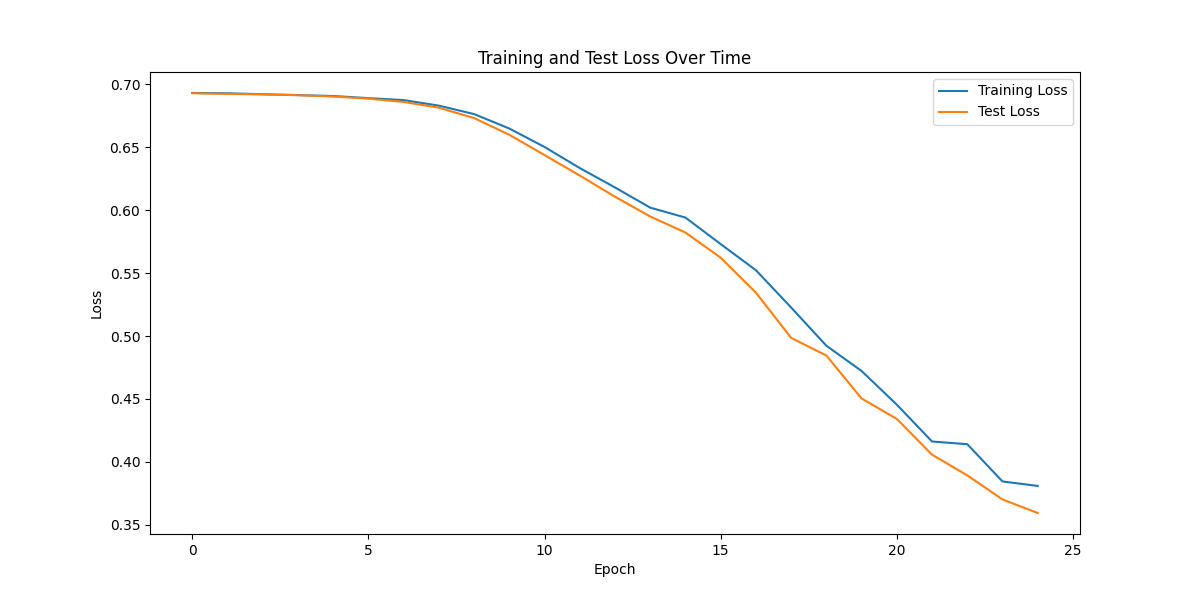
\includegraphics[scale=0.8]{tests/test3_2_e25b32class2_20231211_231613/loss_over_time.png}
  \caption{Gráfico de Perda}
  \label{fig:fig04}
 \end{center}
\end{figure}
